\begin{block}{Outlook - the optical ladder}
  Our group developed compact frequency standards for two differen Cs transitions. Combine this with a frequency comb to get an optical ladder.
  \begin{columns}
    \begin{column}{0.49\textwidth}
     \begin{itemize}
     \item 822 nm reference locks the repetition rate
     \item 884 nm reference lock the absolute frequency
     \item CPT transition provides monitoring of the repetition rate, connecting the microwave and optical regime
     \end{itemize}
    \end{column}
    \begin{column}{0.49\textwidth}
      \begin{figure}
        \begin{center}
          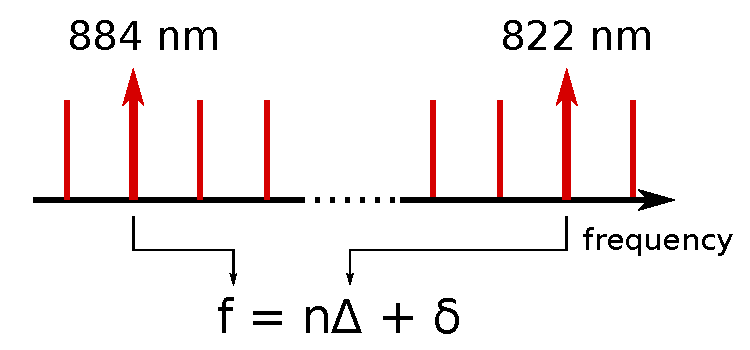
\includegraphics[width=1.0\textwidth]{figures/vernier}
        \end{center}
      \end{figure}
    \end{column}
  \end{columns}
  This scheme removes the need of a highly stable synthetizer, which is an obstacle to a compact and robust design.
\end{block}
